%%%%%%%%%%%%%%%%%%%%%%%%%%%%%%%%%%%%%%%%%%%%%%%%%%%%%%%%%%%%%

\mainmatter
\setcounter{page}{1}

\lectureseries[\course]{\course}

\auth[\lecAuth]{Lecturer: \lecAuth\\ Scribe: \scribe}
\date{December 8, 2009}

\setaddress

% the following hack starts the lecture numbering at 19
\setcounter{lecture}{18}
\setcounter{chapter}{18}

\lecture{Experiment Design \& Model Validation}

\section{Experiment Design}
This lecture corresponds to Part III of Ljung. Experiment design has to do with setting up experiments and designing input signals for a particular system with the goal of getting as much information as possible out of the experiment. Note that the input spectrum, $\Phi_u(\w)$, greatly influences the model fit and can add a bias to the model structure
$$|G_0(\ejw)-G_\theta(\ejw)|^2 \cdot \frac{\Phi_u(\w)}{H_\theta(\ejw)}$$
Typically the input that can be used for a system is constrained such that $|u(t)|<c$. Within this constraint we would like to optimize the information content and the best way is to use white noise where
$$E\{u(t)u(t-\tau)\} = \begin{cases} \mu, & \tau=0 \\ 0, & |\tau|\neq0 \end{cases}$$
but this does not say what $\{u(t)\}$ should actually be.

In \textsc{Matlab} we use \texttt{u = randn(N,1)} to generate a white noise signal. In the case where the input is constrained the high amplitude inputs are not used though. Instead we want to create a white noise signal in the range $[-c,c]$. The solution is to use a pseudo random binary sequence (PRBS) where the input signal is
$$u(t) = \begin{cases} c, & \text{ w.p. } \alpha \\ -c, & \text{ w.p. } 1-\alpha \end{cases}$$
with $0\leq\alpha\leq1$. The pseudo term refers to the fact that the signal generated by the computer will not be truly random on long enough scales due to machine precision and at some point the signal will start to repeat itself.

When we let $\{u(t)\}$ be PRBS in $[-c,c]$ with period $M$ then
\begin{itemize}
\item $\bar{E}\{u(t)\} = \frac{C}{M}$
\item $\bar{E}\{u(t)u(t)\} = \sigma_u^2 = R_u(0) = (1-\frac{1}{M^2})c^2$
\item $\bar{E}\{u(t)u(t-\tau)\} = R_u(\tau) = -\frac{C^2}{M}(1+\frac{1}{M}), \qquad \tau=1,2,\ldots,M-1$
\end{itemize}
A PRBS signal is nearly equivalent to white noise. See Figure \ref{fig:19prbs}.

\begin{figure}[ht!]
	\centering
	\includegraphics[width=.4\textwidth]{images/19prbs}
	\caption{Pseudo random binary input signal.}
	\label{fig:19prbs}
\end{figure}

To capture more low frequency contents the PRBS signal can be held at each value for longer periods. Suppose that $\{e(t)\}$ is a random (normally) distributed signal and let $s(t)=c\cdot\sign(e(t))$ then the signal $s(t)$ is a PRBS in $[-c,c]$ with switching probability $\alpha=0.5$. Then let $u(t)=s(\ent(\frac{t}{N_c}))$ where $\ent(\frac{t}{N_c})$ equals an integer less than or equal to $\frac{t}{N_c}$ and we get
\begin{align}
\label{eq:19ru}
R_u(\tau) = \begin{cases} \frac{N_c-\tau}{N_c}\cdot c^2, & 0\leq\tau\leq N_c \\ 0, & \tau>N_c \end{cases}
\end{align}

\begin{example}
Let $N_c=5$ then $R_u(\tau)$ will not be an impulse response but will look like the dashed line in Figure \ref{fig:19nc}.
$\lozenge$
\end{example}

\begin{figure}[ht!]
	\centering
	\includegraphics[width=.4\textwidth]{images/19nc}
	\caption{Auto covariance with time delays.}
	\label{fig:19nc}
\end{figure}

\section{Frequency Contents of Signal}
Let $\{u(t)\}$ be the signal as defined in (\ref{eq:19ru}), then
$$\Phi_u(\w) = \frac{1}{N_c}\cdot\frac{1-\cos(\w N_c)}{1-\cos\w}$$
and we get a response as in Figure \ref{fig:19fr}. Note that when $N_c=1$ the response is flat because the inverse Fourier transform of an impulse is constant.

\begin{figure}[ht!]
	\centering
	\includegraphics[width=.4\textwidth]{images/19fr}
	\caption{Frequency response of input signal.}
	\label{fig:19fr}
\end{figure}

\section{Alternative Input Signal}
Let $u(t)=F(q)e(t)$ where $\{e(t)\}$ is white noise and $F(q)$ is a stable filter that specifies the desired spectrum, then
$$\Phi_u(\w) = |F(\ejw)|^2\cdot\lambda, \qquad \lambda = R_e(0)$$
Typically $F(q)$ is selected to be a Butterworth filter and $\{e(t)\}$ is set up as white noise with the \texttt{randn} function or as a PRBS with the \texttt{sign(randn)} function in \textsc{Matlab}. Using a second or third order Butterworth filter will produce $\{e(t)\}$ that looks like the signal in Figure \ref{fig:19ripple}. Note that the filter (dashed line) can cause the signal to exceed the constraint $[-c,c]$ but the Butterworth filters are a good choice because they have low damping. Also, filters can be set up to have low or high bandwidth properties.

\begin{figure}[ht!]
	\centering
	\includegraphics[width=.4\textwidth]{images/19ripple}
	\caption{Overshoot of input signal outside of constraints.}
	\label{fig:19ripple}
\end{figure}

\section{Experiment Design for Frequency Domain Analysis}
Using input and output data we can get
$$\{u(t),y(t)\} \Rightarrow \hat{G}(\ejw) = \frac{\hat{\Phi}_{yu}(\w)}{\hat{\Phi}_u(\w)}$$
using ETFE or SPA methods. The underlying technique for all these estimates is the discrete Fourier transform. Recall that
\begin{align*}
\mathcal{S}: y(t) &= G_0(q)u(t) + v(t) \\
\mathcal{M}: Y_N(\w) &= G_0(\ejw)U_N(\w) + V_N(\w) + R_N(\w)
\end{align*}
where $R_N(\w)$ is extra noise in the model. When using periodic input and output signals and performing averaging we have that $R_N(\w)\to0$. The other option is to make the signals ``look'' periodic using approximation techniques such as ``burst'' inputs as shown in Figure \ref{fig:19burst}.

\begin{figure}[ht!]
	\centering
	\includegraphics[width=.4\textwidth]{images/19burst}
	\caption{Burst input where the input signal is very small near the beginning and end.}
	\label{fig:19burst}
\end{figure}

However, an even better method than using a burst input is to use
$$u(t) = \sumk Ak\cos(\w_kt+_\vp k)$$
This is known as a speudo random phase sequence (PRPS). To make the PRPS white let $\vp$ be random in the range $[-\pi,\pi]$ and then take the $N$ time domain points go to $\frac{N}{2}$ points in the frequency domain where $\frac{N}{2}=\frac{\pi}{\dt}$. Then set up the frequency grid such that
$$\w_k = \frac{\pi}{\dt}\cdot\frac{2}{N}\cdot k$$

\section{Model Fit}
For a first order model we get three different possibilities for the number of parameters based on the number of zeros and time delays.
\begin{align*}
G_\theta(q) &= \frac{b_0}{1+a_0q^{-1}}, \qquad H_\theta(q) = 1 \\
G_\theta(q) &= \frac{b_1q^{-1}}{1+a_0q^{-1}}, \qquad H_\theta(q) = 1 \\
G_\theta(q) &= \frac{b_0+b_1q^{-1}}{1+a_0q^{-1}}, \qquad H_\theta(q) = 1
\end{align*}

We will get different values for the prediction error for the different models. More parameters will result in a lower prediction error. The only time to use less parameters is if we have some \textit{a priori} knowledge, for example we know there is a certain time delay or that there are no zeros in the system. Figure \ref{fig:19order} shows what happens as the number of parameters and the model order increases. As $N\gg1$ we will get a perfect fit of the model to the data but it means that we will have modeled the particular realization of noise for that data set.

\begin{figure}[ht!]
	\centering
	\includegraphics[width=.4\textwidth]{images/19order}
	\caption{Prediction error as a function of model order.}
	\label{fig:19order}
\end{figure}

\subsection{Cross Validation}
One way to test whether a model has a good fit for the system is to use one set of data for modeling and a second set of data for validating the model where
\begin{align*}
\mathcal{S}_1: y(t) &= G_\theta(q)u_1(t) + v_1(t) \\
\mathcal{S}_2: y(t) &= G_\theta(q)u_2(t) + v_2(t)
\end{align*}
We can use $\mathcal{S}_1$ to estimate the parameters, $\hat{\theta}$, and then use $\mathcal{S}_2$ to validate the model structure found from $\mathcal{S}_1$. This is known as cross validation and is a good method for model order selection, see Figure \ref{fig:19xvalid}.

\begin{figure}[ht!]
	\centering
	\includegraphics[width=.4\textwidth]{images/19xvalid}
	\caption{Prediction error as a function of model order using model validation.}
	\label{fig:19xvalid}
\end{figure}

\subsection{Validation with One Data Set}
We generally select a model order based on
$$\onen\sumt\est$$
but we can also penalize model order, where $P$ is the number of parameters, to get
\begin{align*}
&\frac{1}{2}\log\left(\onen\sumt\est\right) + \frac{P}{N} \\
&\frac{1+\frac{P}{N}}{1-\frac{P}{N}}\cdot\onen\sumt\est
\end{align*}
The first equation is known as Akaike's Information Criterion (AIC) and the second equation is Akaike's Final Prediction Error Criterion (FPE) and both criterion functions are available in \textsc{Matlab}. Note that it is better to split the data and perform cross validation if that is possible.

\section{Model Validation}
To determine whether a model is good enough depends on the application. For control applications we can use the small gain theorem (see \S\ref{sec:15sgt}) where we want
$$\left|\left|\Delta\cdot\frac{C}{1+\hat{G}C}\right|\right|_\infty < 1$$

For prediction we can check to see if $\{\ett\}$ is white noise.

For simulation we have
$$\ett = H_\theta^{-1}(q)(y(t)-G_\theta(q)u(t))$$
and we can check to see if $R_{\epsilon u}(\tau)=0 ~\forall \tau$ to find out if the input is uncorrelated with the prediction error.

In terms of difficulty prediction is the most difficult, control is the least difficult and simulation is somewhere between those two.

\subsection{Validating System Model}
We can determine whether the system has been modeled by checking $R_\epsilon(\tau)=0$ for $|\tau|>0$ and at $\tau=0$ we get the variance. In practice we have to replace this with $\hat{R}_\epsilon(\tau)=0$ and since this is an estimate it should be done with confidence intervals. What typically occurs is we get
$$\sqrt{N}\cdot\frac{\hat{R}_\epsilon^N(\tau)}{\hat{R}_\epsilon^N(0)} \sim \mathcal{N}(0,1)$$

\subsection{Validating Noise Model}
To determine if the noise has been modeled correctly we can check $R_{\epsilon u}(\tau)=0$. Then we get
\begin{align*}
&\sqrt{N}\hat{R}_{\epsilon u}(\tau) \sim \mathcal{N}(0,P) \\
&P = \sum_{k=-\infty}^\infty R_\epsilon(k)R_u(k)
\end{align*}
Again, we need to use confidence intervals because we are using estimates where the confidence bars are placed at intervals based on the variance of the signal, such as at $3\sigma$ levels for $99\%$ confidence.
%%%%%%%%%%%%%%%%%%%%%%%%%%%%%%%%%%%%%%%%%%%%%%%%%%%%%%%%%%%%%